\chapter{Background}\label{chp:background} 
\chapterprecishere{"We model the future on the past. Sometimes that’s a mistake."\par\raggedleft--- \textup{Van Jacobsen}, SIGCOMM 2001}

This chapter will give a brief overlook of the motivation for \gls{ICN},
as well as explaining more details of \gls{ICN} protocols such as \gls{CCN} and \gls{NDN}.
The \gls{NDN} architecture will be reviewed.
Finally a quick summary of related works.

\section{Motivation for Information-Centric Networking}
When Internet was created in the 1960's, the researchers where inspired by the existing communication network; the telecommunication network.
Because it was natural and logical to think that people would send and receive short messages and instructions, the point-to-point communication model was a logical architecture. 
As Internet have developed, the traffic has increased enormously over the past few years. 
In the Global Internet Phenomena Report 1H2014 done by Sandvine~\cite{gipr2014}, close to 64\% of all \gls{IP} traffic in North America was Real-Time Entertainment streaming.
In~\autoref{fig:ip-traffic} it can easily be seen that most of the traffic is content download, and not communication.
With this in mind, the \gls{IP} architecture does not provide an efficient transport model for what we are actually using the network for.

\begin{figure}[ht]
  \centering
  \begin{subfigure}{0.48\textwidth}
    \centering
    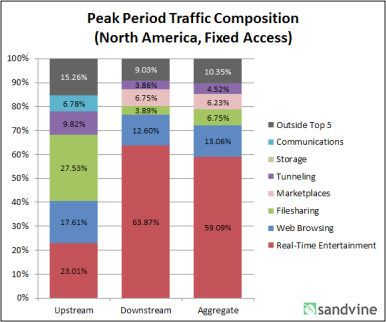
\includegraphics[width=1\linewidth]{north-america-ip-traffic.png}
    \caption{North America}
    \label{fig:north-america-ip-traffic}
  \end{subfigure}

  \begin{subfigure}{0.48\textwidth}
    \centering
    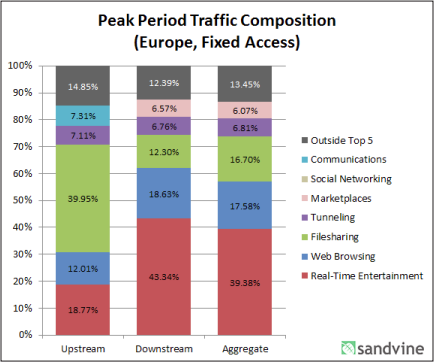
\includegraphics[width=1\linewidth]{europe-ip-traffic.png}
    \caption{Europe}
    \label{fig:europe-ip-traffic}
  \end{subfigure}
  \caption{
  (a) Peak Period Aggregate Traffic Composition - North America, Fixed Access~\cite{gipr2014}.
  (b) Peak Period Aggregate Traffic Composition - Europe, Fixed Access~\cite{gipr2014}.
  }
  \label{fig:ip-traffic}
\end{figure}

Designing the \gls{IP} network, the security was not the first priority.
A logical though considering that they did not know what the Internet was going to be used for and how big it has become.
Most of the protocols related to Internet have been designed and deployed mainly with the goal of functionality to work.
In the years after the birth of Internet, they soon found out that they needed security at several layers, due to that the application requirements and the transmission importance increased.
\gls{IPsec} is a very good example of work trying to patch up security flaws in Internet.

Today, WiFi is disseminated across homes and buildings in many countries. 
Wireless technology has grown rapidly and it is predicted continuous growth in the years to come.\todo{find a cite} 
The \gls{IoT} trend is coming, and the \gls{IP} network is not designed for broadcast and therefore wireless connection is not as easy as it should be.
Devices should easily be able to communicate directly with each other without having to interconnect through a router.

Another problem is the network redundancy. 
Looking at~\autoref{fig:ip-traffic} one can conclude that there are a lot of movies downloaded from \textit{x} users geographically located close, and thus the network path from the source (e.g. Netflix) to this geographical place is allocated \textit{x} too many times. 
This is due to that a node in an \gls{IP} network does not know \textit{what} it processes, but rather the packet's endpoints, i.e. \textit{where} it goes and \textit{where} it comes from. 
This makes every node dumb, hence the network is designed for redundancy when it comes to content download.

These design failures are some the reasons why the research for Future Internet began.  
\gls{ICN}~\cite{DBLP:journals/cm/AhlgrenDIKO12} is a concept developed under this research.
It is built upon delivery of content, rather than the point-to-point model we previously have seen.
\gls{ICN}s goal is to build an infrastructure of a new Internet that can achieve efficient, secure and reliable distribution of content.
In 2012 \gls{IRTF} established \gls{ICN} working group.


\section{Content Centric Network \& Named Data Network}\label{chp2:sec:icn}
The first network protocol purposed for \gls{ICN}, \gls{CCN}, was presented by Van Jacobsen at a Google Talk in 2006. 
He, amongst other contributors of \gls{CCN}, has been working on developing the Internet as we know it since the early start.
Jacobsen has contributed to \gls{TCP}/\gls{IP} with his flow control algorithms and \gls{TCP} header compression. \todo{cite}

\gls{CCN} focuses on naming content, instead of naming \gls{IP}-addresses. 
The research project is lead by \gls{PARC}.
A branch of \gls{CCN} is the \gls{NDN}~\cite{DBLP:journals/ccr/0001ABJcCPWZ14} research project started in 2010, which Jacobsen also have contributed to.
One of the biggest contributers is \gls{UCLA}, with Lixia Zhang in the lead. 
The \gls{NDN} project is also one of few projects selected by \gls{NSF} \gls{FIA} program~\cite{nsf-fia}.

\section{NDN Architecture}\label{chp2:sec:ndn_architecture}
Since the knowledge of how \gls{NDN} works is not disseminated amongst computer scientists, it is essential for this paper to describe how it works.
This section will describe the basic architecture of \gls{NDN}~\cite{NDN-0021} and compare some solutions with the equivalent solutions in \gls{IP}.
\subsection{Brief Introduction}
\todo{a section explaining NDN briefly so the reader has something to relate to reading the following sections}

\subsection{Based on Existing Solution}
The goal for the network design is essentially making it more applicable for content without removing the communication service that \gls{IP} was designed for. 
Designing a new network protocol we have to look at what measurements we have done in the existing \gls{IP} network to tailor it towards content sharing.
As the reader might notice after reading the background material, \gls{NDN} is built upon concepts that we can map to well working solutions from deployed over \gls{TCP}/\gls{IP}.
Some examples are:
\begin{itemize}
  \item BitTorrent - 
  The concept of sharing bits of files between peers in a network is a well-working distributed method for sharing content.
  \item \gls{CDN} - 
  Many \gls{ASP}s, such as Netflix and YouTube, have found out that the \gls{IP} network performs a lot better for their costumers if they cache up their data.
\end{itemize}

Namespace-based trust introduced in \gls{SDSI}, binding names to public keys. \todo{write something about this}

\subsection{Packets}\label{packets}
There is two types of packets in \gls{NDN};
\textit{Interest packet} and the corresponding answer, i.e. the \textit{Data packet}, illustrated in~\autoref{fig:packets}.

\begin{figure}[H]
  \centering
  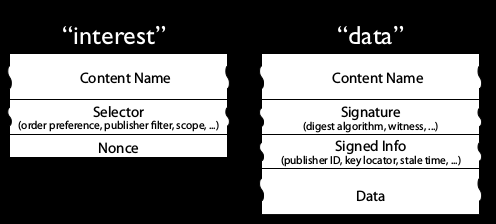
\includegraphics[width=1\textwidth]{packets.png}
  \caption{Interest packet and Data packet}
  \label{fig:packets}
\end{figure}

The Interest packet specifies a Content Name. 
The Name can have a hierarchical structure and signatures can be added after the \gls{URI}, e.g. ``/ndn/no/ntnu/haakon/file/1/<signature>''.
An Interest can also contain a set of different Selectors to specify original requirements for the Data response. 
Some of the Selector fields are:
\begin{itemize}
  \item KeyLocator - can be used to specify where the Public Key for the signature can be found.
  \item Exclude - can be used to specify a list or a range of names that should be excluded from the Name. 
  I.e. if the Name is ``/ndn/no/ntnu'' and the Exclude contains ``/item'', the returned Data does not contain ``/ndn/no/ntnu/item''.
  \item MustBeFresh - if True, a node cannot answer with a Data packet where the FreshnessPeriod has expired.
  \item ChildSelector - can be used to select either the leftmost (least) or the rightmost (greatest) child, e.g. content version. 
  \item Min/MaxSuffixComponents - refers to name components that occur in the matching Data beyond the prefix. 
\end{itemize}
The Nonce field sets automatically. 
This is used to uniquely identify an Interest and prevent looping in the network.

The Data packet it a response to the Interest packet, and contains the Content Name and the Content itself.
It also has a MetaInfo field that is used to specify the FreshnessPeriod (milliseconds), ContentType and FinalBlockId. 
Now when somebody requests a file ``/ndn/no/ntnu/haakon/file/1'' with an Interest, the response will have the same name, but also containing the file.

Because only a Data packet can exists if there is a corresponding Interest, \gls{NDN} is pull-based.
Hence unsolicited Data packets will be thrown away, i.e. there is no content in the network, that is not requested from someone.
This reduces unwanted traffic compared to \gls{UDP} in \gls{IP}, and minimizes the \gls{DoS} vulnerability drastically.

\subsection{Names}\label{name}
In the \gls{NDN} network there is no strict rules for a Name.
This means that a network node only routes an Interest based on longest prefix match.
Naming is left to the application design, thus it can be customized for the applications best purpose.
However the network assumes hierarchical structured names, hence routing will perform better with a hierarchical name design.

For the network to perform even better, the Interest can append some Selectors that can help the network to decide which Data to retrieve and where to route.
With Selectors a partially known name can successfully retrieve the right Data.
E.g. when a user want to download the newest version of some content, lets say ``/ndn/no/ntnu/haakon/file/<version?>'', but do not know which version is the newest, the user can append a ChildSelector to choose the greatest version.

When designing applications for the \gls{NDN} network, one might learn from \gls{DNS} and \gls{OS} naming.
\todo{write more}

\subsection{Network Node}
If we look at an existing model of an \gls{IP} node~\autoref{fig:ip-model-node} and compare it to a \gls{NDN} node~\autoref{fig:icn-model-node}, we see that they look much the same.
However, the logic behind a \gls{NDN} node is a bit more complex, and thus lead to more knowledge about \textit{what} content the node has to offer.
To understand this, the following entities in a \gls{NDN} node should be understood:
\begin{enumerate}\label{ndn-node-modules}
  \item Face - A term used for generalization of different interfaces, e.g. physical like Ethernet, or overlay like \gls{TCP} and \gls{UDP}. A Face can also be a UNIX-domain socket for communication with a local application.
  \item \gls{PIT} - All pending or recently satisfied Interests are stored here, together with the incoming and outgoing Face.
  If a new incoming Interest matches a entry in the \gls{PIT}, the incoming Face will be added to the entry. 
  \item \gls{CS} - When a node receives a Data packet that has the corresponding entry in the \gls{PIT}, it stores the Data packet in \gls{CS} as long as possible. 
  \item \gls{FIB} - Forwarding strategy is stored for each Name prefix. 
  When a node forwards an Interest, it will do a longest prefix lookup in the \gls{FIB} and send the Interest further to the best matching Face.
\end{enumerate}

\begin{figure}[H]
  \centering
  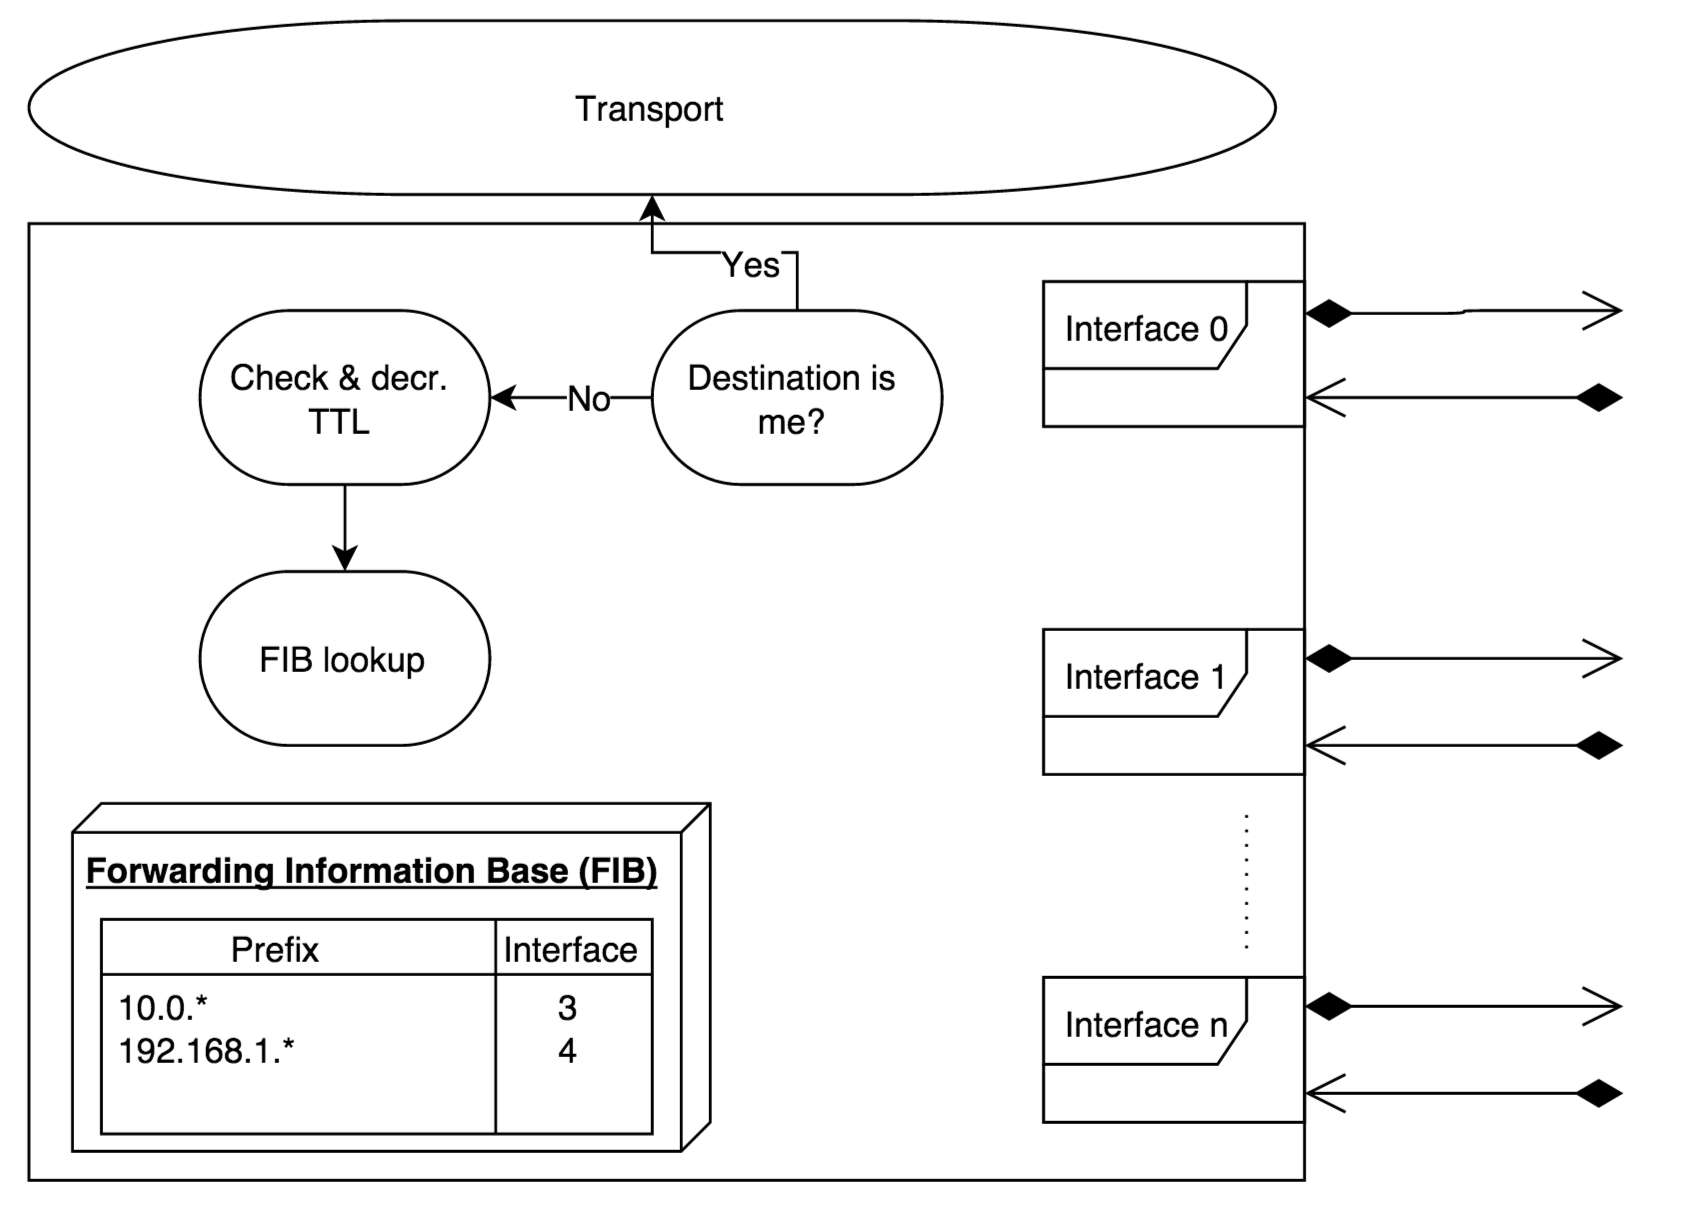
\includegraphics[width=0.8\textwidth]{ip_model_node.png}
  \caption{Model of IP node. A packets enters the node through an Face. 
  The node decides whether the packet is for the node itself, or passes it further to next node, found in the FIB.}
  \label{fig:ip-model-node}
\end{figure}

\begin{figure}[H]
  \centering
  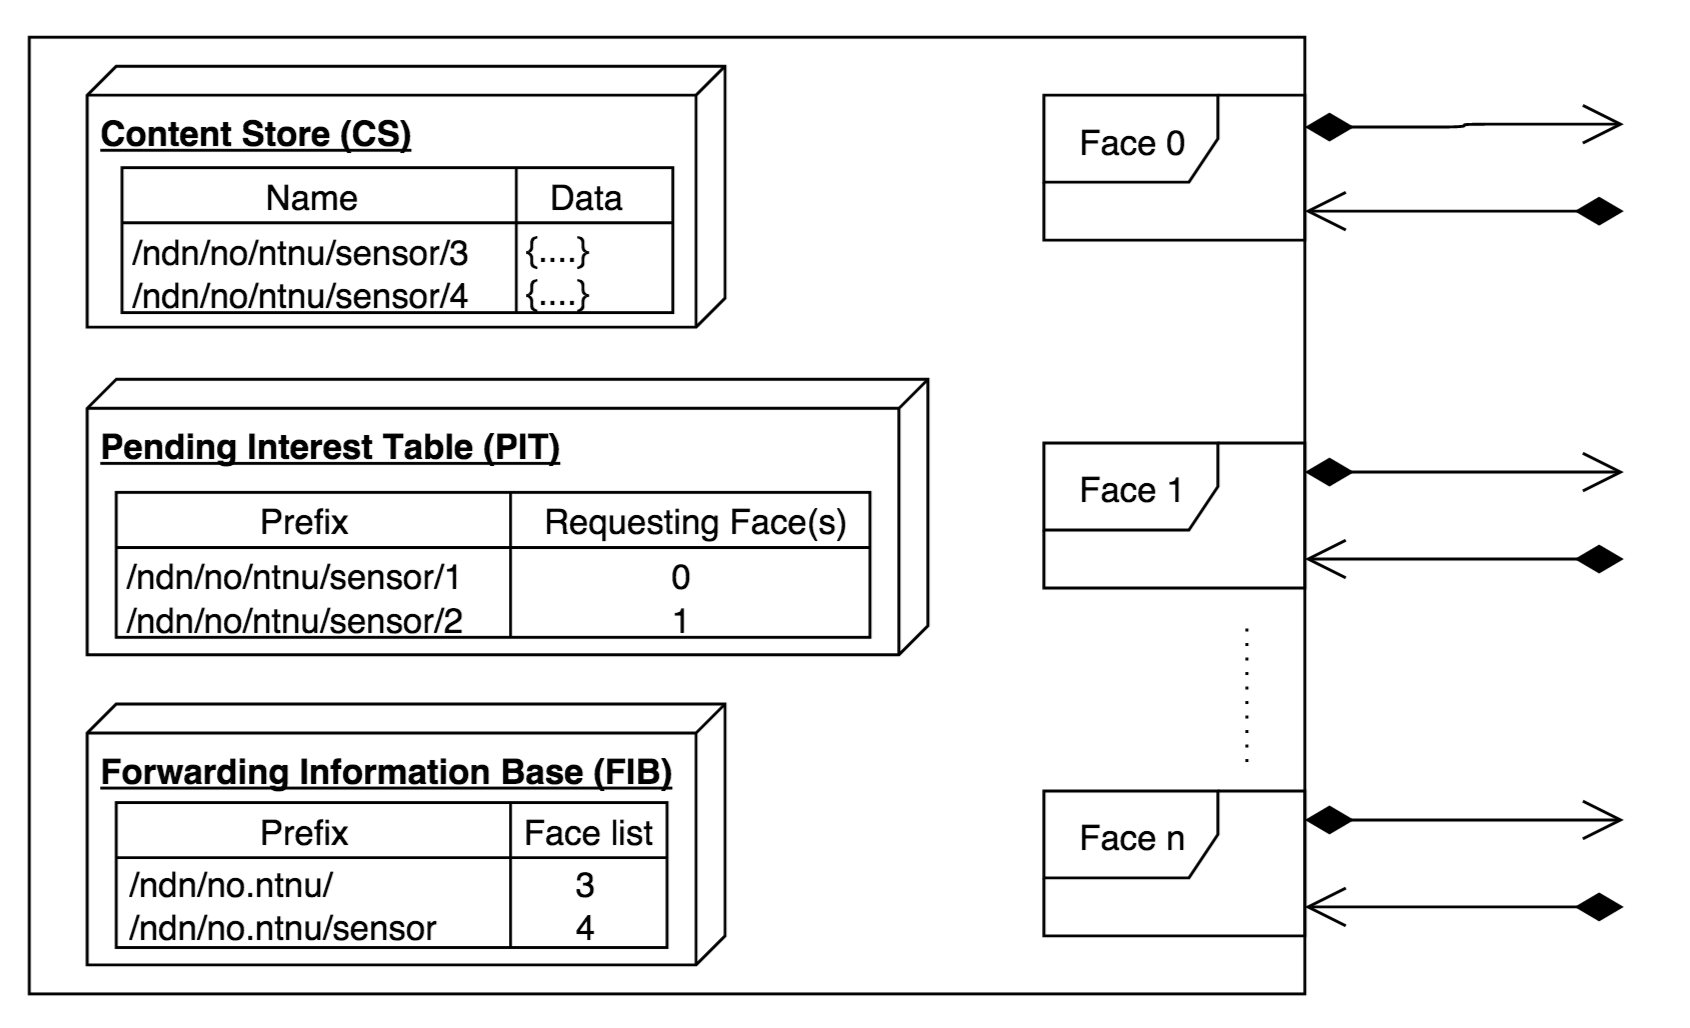
\includegraphics[width=0.8\textwidth]{icn_model_node.png}
  \caption{Model of NDN node. A packet enters through an Face. 
  The node checks whether the Interest is already queried in the PIT, or stored in the CS, or passes it further to next node, found in the FIB.}
  \label{fig:icn-model-node}
\end{figure}

In contrary to an \gls{IP} node, a \gls{NDN} node knows \textit{what} content comes through itself. 
Since all content is associated with a Name, a \gls{NDN} node can know 1) \textit{what} is requested, but not satisfied (i.e. \gls{PIT}), and 2) \textit{what} has been satisfied earlier and still available, i.e. still cached in\gls{CS}.
With this ability the network can now supply requests with content already stored in cache, hence the network can naturally offer multicast.
\todo{Unicast (TcpFace, UdpFace) vs Multicast (MulticastUdp, Ethernet)}
~\autoref{fig:ndn-multicast} illustrates a \gls{NDN} network where we can see that the network does not nearly have to send equal amount of traffic than in an \gls{IP} network.
The mobile expresses an Interest (1) in a file named \path{/ntnu/file1}.
The Interest finds its way to the publisher of the file, and thus the publisher responds with a Data packet (2) named \path{/ntnu/file1} containing the file.
When the second computer expresses the same Interest (3), the consecutive node already has cached the Data response matching to the Interest in its \gls{CS}, hence the Interest is satisfied already at this point, and not forwarded any further.
Same happens when the third computer expresses again the same Interest (4) to the network.
Given that the file these computers are interested in is 4 gigabyte, the network saves a lot of traffic with multicast.
\begin{figure}[H]
  \centering
  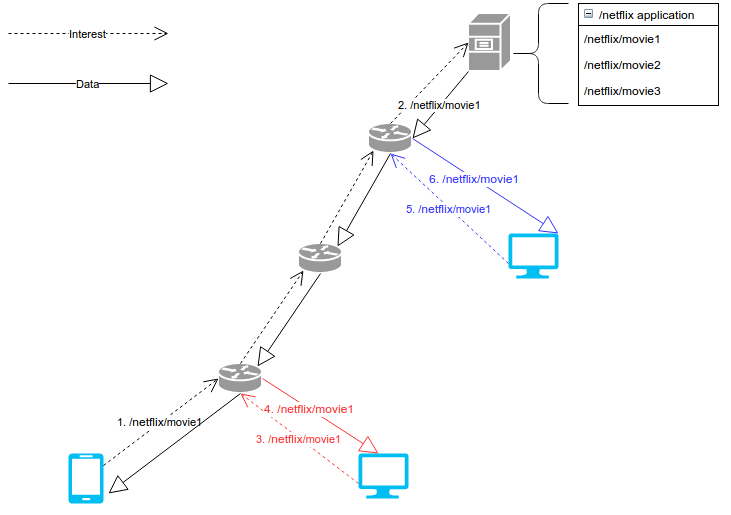
\includegraphics[width=1\textwidth]{ndn-multicast.png}
  \caption{Multicast in NDN.}
  \label{fig:ndn-multicast}
\end{figure}
 
\subsection{Incoming Interest}\label{incoming-interest}
In~\autoref{fig:icn-model-node-decision-interest} we see an incoming Interest through a Face. 
The node checks the \gls{PIT} for pending or recently satisfied Interests. 
If there is no match, the node will do a lookup in \gls{CS} to see if a corresponding Data packet is cached. 
If there is a match in the \gls{PIT} it will only add the Face to the \gls{PIT} entry. If there is a match in the \gls{CS} the node will return the Data. 
If there is no match in either the \gls{PIT} or the \gls{CS} the node will make a new \gls{PIT} entry and do a longest prefix match lookup in the \gls{FIB} to decide which Face(s) to forward the Interest. 
How to forward a Interest; routing strategy. 
A strategy per \gls{PIT} entry. 
I.e. whether, when, and where to forward the Interest.
\begin{figure}[H]
  \centering
  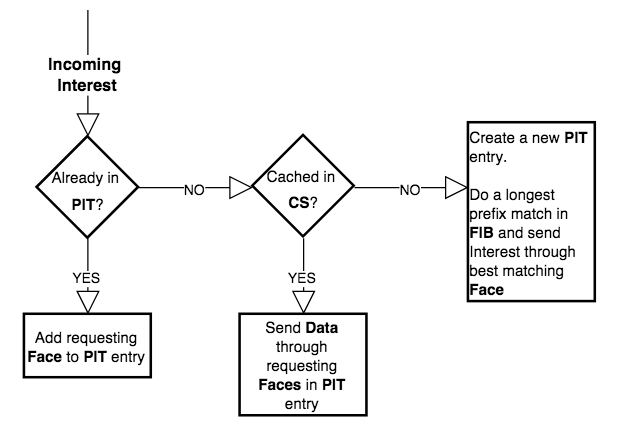
\includegraphics[width=1\textwidth]{ndn-node-decision-tree-interest.png}
  \caption{Decision tree for a NDN node when receiving an Interest.}
  \label{fig:icn-model-node-decision-interest}
\end{figure}

\subsection{Incoming Data}
In~\autoref{fig:icn-model-node-decision-data} we see incoming Data.
The node will check  the \gls{PIT} for an entry, if a match is found the node will forward the data to all the Faces registered in the \gls{PIT} entry.
The node checks the data from local applications cached in \gls{CS} first, if there is no match, it stores the content in \gls{CS} and sends the data to all requesters (i.e. through all Faces stored in the \gls{PIT} entry).
\begin{figure}[H]
  \centering
  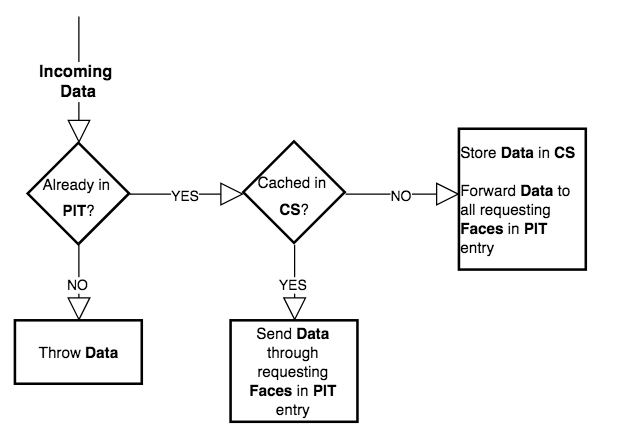
\includegraphics[width=1\textwidth]{ndn-node-decision-tree-data.png}
  \caption{Decision tree for a NDN node when receiving Data.}
  \label{fig:icn-model-node-decision-data}
\end{figure}


\subsection{Security}\label{ndn-security}
Below I will present why \gls{NDN} facilitates good security properties, explaining some of the security aspects around \gls{NDN} discussed in~\cite{secure-network-content}, and the difference in securing data and securing channel.

\todo{this section needs to be refactored}

\subsubsection{Trusting Host vs Trusting Content}
The \gls{IP} network is designed in a way that makes us wanting to trust the host.
What we actually are trusting is the mapping of the \gls{URL} to the \gls{IP} address.
It is not a good security model doing a whole lot of mapping at different layers, since each mapping introduces a potentially vulnerable target for forgery.
\gls{DNS} points to a host address that speaks for the \gls{URL} you are interested in, and thus if someone manages to forge this address, you cannot tell if you talk to the right host.

The content is rarely encrypted and the confidentiality is not preserved, unless there is established a secure channel using e.g. \gls{TLS}.
This is a problem due to the issues concerning tampering and eavesdropping.
The content the host we trust provides can contain malicious software and important information can be swapped. 
The solution is to encrypt the connection. 
This is the concept of securing the channel, and the trust is based on certificates.
Due to the global \gls{PKI} and essentially because the certificate is signed by a \gls{TTP} all trust comes outside the namespace.
This makes it problematic over \gls{IP} to retrieve content from other than the trusted host because you do not trust any other than the host you are connected to via the secure channel.

A goal is to get the desired content from the intended source, unmodified in transit.
Therefore a better solution would be to trust the content rather than the host.
This concept requires us to change the network trust.
Skipping 1) all the trust based in mapping of hosts, 2) where the data comes from, and 3) securing the channel.
The content should be linked to the publisher and this linkage should be signed by the publisher. 
The concept is to mathematically prove that the content originates from the believed publisher, and that its not modified nor been exposed to unauthorized eyes (if necessary).
This introduces a possibility that anyone can retrieve any piece of data from anyone regardless of secure channel or not.
How can this idea be achieved? 
As Diana Smetters and Van Jacobsen says~\cite{secure-network-content}, we must ensure the content's validity, provenance and relevance.

\begin{itemize}
  \item Validity - Complete and unmodified content from the publisher.
  \item Provenance - Should the publisher be trusted with the content requested?
  \item Relevance - Is the content what the requester intended?
\end{itemize}

One can do hash verification on the content to be sure that the content is unmodified. 
But there should be a binding between the Name to the content.
However this does not provide provenance nor relevance.
For this there should be a linkage between the publisher, the Name and the content.
Doing a triple mapping of the Name (N) and content (C), cryptographically signed by the publisher (P) seen in~\autoref{eq:mapping_name-content}.
This mapping is unique, relying on the hash computation done in the signing, and it provides validity, provenance and relevance.
A requester can easily verify the Name and content binding, as well as authenticating that the data originates from the publisher who knows what the content is.
Now anybody can retrieve \texttt{M\textsubscript{(N,P,C)}}, hence an untrusted host and an insecure channel is not so bad anymore.

\begin{equation}\label{eq:mapping_name-content}
M_{(N, P, C)} = (N,C,Sign_{P}(N,C))
\end{equation}

A clear benefit of this approach is that the Name can be of any form. 
Different naming rules should apply for different applications as there are no global naming rules that are optimal for each application.

This concept is integrated in the \gls{NDN} protocol and it is required that every packet delivered from application layer is signed by the application.
The protocol also provides an easy way for the application to encrypt data providing confidentiality.
Encrypting the content with symmetric keys that are distributed to parties obtaining access right to the content together with the validity, provenance and relevance provides a way of securing data rather than securing communication channels.

\subsubsection{Anonymity}
% TOR network
Based on the nature of this architecture, \gls{NDN} facilitates the practice of anonymity in the network. 
In a Tor network~\cite{DBLP:conf/uss/DingledineMS04}, each node participating in a circuit only knows the two neighboring nodes.
Only a ``Global passive adversary'' that can monitor the whole network is able to decide the whole packet path, hence know \textit{who} is requesting and \textit{who} is responding.
Since the packet format (\autoref{packets}) in \gls{NDN} has no source or destination specific field as in a \gls{IP} packet, the privacy of the network is more similar to a Tor network.
If a packet is captured at any arbitrary point of its path, the only information an adversary will get, is the two nodes between the packet capture and the data name. 
Unless monitoring a complete network, it should be close to impossible to track packets.  
However because of the semantic naming there are some issues related to privacy as it easily can be seen in the Name \textit{what} the content contains in many cases.
Also since signing of each Interest is required by the sender, some privacy information might leak.
DiBenedetto et al. try to address these problems in~\cite{DBLP:conf/ndss/DiBenedettoGTU12} with an approach that use existing solutions from the Tor network.
In 2010 the \gls{NDN}-team planned to implement TORNADO~\cite[Section 3.7]{NDN-0001}, the \gls{NDN} version of Tor, to demonstrate the privacy preservation capability of the network.

\todo{more in this section}

\section{Attacks}

Paolo Gasti et al. identifies several \gls{DoS} attacks on \gls{NDN} in their paper about \gls{DoS} \& \gls{DDoS} in \gls{NDN} ~\cite{DBLP:conf/icccn/GastiTU013}. Other works have been done related to \gls{DoS} in \gls{NDN}~\cite{DBLP:journals/ijcomsys/WangCZQZ14, DBLP:conf/ancs/SoNO13, DBLP:journals/corr/abs-1303-4823}

In~\cite{DBLP:journals/tifs/LiZZSF15} Zhang et al. proposes an extension of the \gls{NDN} protocol for addressing the access problem of cached data in nodes.  
The \gls{NDN} network is also potentially susceptible to content poisoning attacks which Ghali et al. addresses in~\cite{DBLP:journals/ccr/GhaliTU14}.

\section{Related work}
The work in this thesis builds upon three main concepts; synchronization, sensor networking and \gls{IBC}. 
Some related work done will shortly be presented in this section.

\subsection{Synchronization}
Synchronization application over \gls{NDN} called iSync~\cite{DBLP:conf/acmicn/FuAC14}.
A synchronization application build by the \gls{NDN} team is ChronoSync~\cite{DBLP:conf/icnp/ZhuA13}.

\subsection{Secure Data Retrieval from Sensors}
Amadeo et al.~\cite{DBLP:conf/acmicn/AmadeoCM14} proposes a solution for reliable retrieval of data from different wireless producers which can answer to the same Interest packet. This is highly applicable to a sensor network where you want to communicate with closest sensor, e.g. the light in \textit{this} room.
In~\cite{DBLP:conf/noms/AbidySLF14} Abid et al. simulate data aggregation in wireless sensor networks.
Burke et al. addresses efficient and secure Sensing over \gls{NDN} in~\cite{DBLP:conf/nca/BurkeGNT14}

Securing Building Management Systems Using Named Data Networking~\cite{DBLP:journals/network/ShangDMBZ14}

\subsection{Identity-Based Cryptography in Named Data Networking}
There is done some research with \gls{IBC} in \gls{NDN}. In~\cite{DBLP:conf/icnp/ZhangCXWSW11} Zhang et al. proposes a hybrid scheme with traditional \gls{PKI} and \gls{IBC}.


\todo{write more, mer utfyllende}